%=====================================================================
\chapter{Metodologia} \label{chp:metod}
%=====================================================================

O fluxo de trabalho adotado incluiu etapas de estudo do problema e das ferramentas disponíveis para tratá-lo, definição de critérios de análise para a tomada de decisão entre as opções disponíveis, planejamento de testes comparativos e codificação de um programa com interface de linha de comando para concretizar uma solução minimamente viável que possa ser integrada ao Projeto E-Foto em suas versões futuras.

\section{Estudo do cenário}

Entre os objetos a serem estudados para a confecção do trabalho destacam-se o levantamento das necessidade do software (e-foto), das ferramentas computacionais que implementam partes essenciais da solução e dos conjuntos de dados disponíveis para realização de testes.

\subsection{Levantamento das necessidades do e-foto}

No início do projeto, foi considerado o estado atual do software levando em consideração atualizações não publicadas aos usuários, seja por meio de suas documentações ou de seus lançamentos de versões executáveis, mais de conhecimento dos principais desenvolvedores ativos no projeto. Foram identificados ainda quais módulos se beneficiariam das possíveis respostas deste trabalho e escolhido um módulo alvo, como prova de conceito. 

Para tal, foi preciso realizar um análise mais aprofundada destes módulos visando o entendimento dos dados que eles necessitam para funcionar e como estes são entregues. O alvo escolhido foi aquele com menor dependência de acoplamento, isto é, que permite o mínimo de alteração no software, atuando assim como um provedor de dados isolado a ser integrado posteriormente ao considerar uso dos formatos de arquivos suportados atualmente. 

Cabe ressaltar que existe um método pouco documentado do e-foto, elaborado especificamente para o desenvolvimento e testes do módulo de aerotriangulação \cite{pupim2012}, que permite a importação de pontos através de 2 arquivos de texto ``.txt". Estes arquivos são preenchidos com as informações de ENH dos pontos, ou seja, suas informações geográficas, e a localização desses pontos quando medidos nas imagens. Isto possibilitou o foco do trabalho na comparação de técnicas, deixando para o software conjuntos de dados que possam ser importados em seu ambiente.

O módulo alvo escolhido realiza a aerotriangulação. Ele adota pontos fotogramétricos, que equivalem aos pontos de costura até o momento em que o módulo efetua seus cálculos, pois estes pontos adquirem coordenadas de terreno como consequência do processo de ajustamento do bloco de imagens. Atualmente estes pontos devem ser medidos manualmente nos conjuntos de imagens de um bloco fotogramétrico, antes que o processo possa ser executado.

Dentre as opções deixadas fora do escopo deste trabalho, mas consideradas na etapa de estudos, estão os módulos de restituição estereoscópica e de extração de modelos digitais de superfície. Ressalta-se que estes módulos não poderiam ser abastecidos com os dados deste trabalho sem alteração direta do e-foto. Contudo, os resultados da fase de estudo para estes módulos serão compartilhadas no Capítulo \ref{results} como referências para trabalhos futuros. Outra opção, também descartada, foi a confecção de um novo módulo completo para seleção de pares e visualização de foto-índices. Mais uma vez, cabe ressaltar que este trabalho pode ser considerado como uma das bases para o novo módulo.
 

\subsection{Seleção de ferramentas aplicáveis na solução}

Foram consideradas as bibliotecas de visão computacional que ofertassem métodos para detecção e descrição de pontos chaves, bem como para realizar correlação de feições e correções geométricas. Uma qualidade avaliada foi a portabilidade, ou seja, capacidade de funcionar nos principais sistemas operacionais da atualidade. Também foram consideradas as linguagens de programação disponíveis para que os resultados pudessem ser incorporados ao e-foto futuramente.

Muitas opções de APIs (interfaces de programação de aplicações) para visão computacional foram publicadas nos últimos anos. Desde opções abertas à comunidade desenvolvedora como é o caso de 
OpenCV (apresentada em detalhes no Capítulo \ref{chp:fund}),
SimpleCV\footnote{SimpleCV: plataforma de aplicativos de visão computacional em Python disponível em \url{https://simplecv.org}},
BoofCV\footnote{BoofCV: biblioteca aberta de visão computacional de tempo real em Java disponível em \url{https://boofcv.org/}} e
Scikit-image\footnote{Scikit-image: coleção de algoritmos para processamento de imagens elaborados pela comunidade Python disponível em \url{https://scikit-image.org}},
até soluções corporativas em redes, como é o caso da Amazon 
\footnote{AWS Rekognition disponível em \url{https://aws.amazon.com/pt/rekognition}}, 
da Google\footnote{Google Cloud Vision disponível em \url{https://cloud.google.com/vision}}
e da Microsoft\footnote{Azure Computer Vision disponível em \url{https://azure.microsoft.com/en-us/services/cognitive-services/computer-vision}}.
Dentre tantas opções, merecem destaque o Orfeo-Toolbox e o Opticks, pois tratam-se de projetos de código aberto focados no processamento de imagens de sensoriamento remoto com suporte da Open Source Geospatial Foundation (OSGeo), uma organização sem fins lucrativos cuja missão é promover a adoção de tecnologias geoespaciais abertas à comunidade. 

Optou-se por utilizar neste trabalho o OpenCV, uma das mais completas bibliotecas de visão computacional, pois ela é desenvolvida em linguagem C++ (tendo usado interface em C até sua versão 2.4), além de possuir um número considerável de exemplos. Ela é também base para outros aplicativos de processamento de imagens aéreas como o 
Open Drone Maps\footnote{Software com código disponível em \url{https://github.com/OpenDroneMap/} que depende de OpenSFM hospedado em \url{https://github.com/mapillary/OpenSfM}} (ODM).

Outras características interessantes do OpenCV são uma boa portabilidade entre sistemas operacionais, além de interfaces com outras linguagens de programação como o Python, permitindo assim seu uso na extensão de aplicações. Deste modo, entende-se que ela se alinha com critérios básicos de seleção de dependências para o e-foto e pode vir a ser uma ferramenta de apoio em suas versões futuras. Logo, estima-se que tal escolha auxilie na integração dos resultados com o e-foto, mesmo considerando diferentes cenários de curso do seu desenvolvimento, principalmente por este também ser desenvolvido utilizando-se da linguagem C++, mas também por este já adotar chamadas para outros programas de linha de comando, como o \textit{xsltproc} \cite{jonas2012} e pelo potencial para a adesão de novos alunos ao projeto interessados em trabalhar com outras linguagens de programação.

A versão escolhida de OpenCV foi a 4.5.4, que não é a versão mais recente da biblioteca, mas inclui diversas melhorias consideradas importantes neste trabalho. O principal motivador para a escolha da versão foi a observação de que os repositórios de arquivos binários para diversas distribuições Linux já dispõem desta versão\footnote{Para mais informações acesse \url{https://repology.org/project/opencv/versions}}. Ela ainda pode ser utilizada em Windows e Mac através de binários disponibilizados em repositórios do tipo Conda\footnote{Disponível em \url{https://anaconda.org/conda-forge/libopencv}}.

Em OpenCV estão muitos dos trabalhos mais recentes de pesquisa da área de visão computacional. No que toca este trabalho, a Tabela \ref{Feature2D} indica os algoritmos do módulo de análise de feições em 2D, disponíveis na versão escolhida da biblioteca. São listadas as implementações disponíveis para diferentes algoritmos de detecção e descrição de feições, indicando onde estes se aplicam. Em grande parte as classes disponíveis são consideradas experimentais ou possuem patentes atreladas ainda vigentes e, por este motivo, tais algoritmos são isolados na extensão ``xfeatures2d'' que implica em dependência de códigos de terceiros. Outra dependência comum a algumas partes desta biblioteca é o ``CUDA'' ( acrônimo de \textit{Computer Unified Device Architecture}), que é uma arquitetura de processamento paralelo de propósito geral desenvolvida pela NVIDIA permitindo uso de suas placas de video (GPUs). O uso de processamento paralelo pode reduzir o tempo de resposta de sistemas, porém aumenta significativamente o custo de equipamentos compatíveis. Neste sentido, para o Projeto E-Foto desconsideramos no trabalho o uso de quaisquer recurso CUDA e da maioria dos algoritmos considerados experimentais.

\begin{table}[!ht]{12cm}
  \caption{Implementações da interface Feature2D}\label{Feature2D}
  \hfill
  \begin{tabular}{l|c|c|c}
    \hline
      Algoritmo & Detecção & Descrição & Dependência \\
    \hline
      AffineFeature & \cmark & \cmark & -\\
      AgastFeatureDetector & \cmark & \xmark & -\\
      Akaze & \cmark & \cmark & -\\
      BRISK & \cmark & \cmark & -\\
      FastFeatureDetector & \cmark & \xmark & -\\
      GFTTDetector & \cmark & \xmark & -\\
      KAZE & \cmark & \cmark & -\\
      MSER & \cmark & \xmark & -\\
      ORB & \cmark & \cmark & -\\
      SIFT & \cmark & \cmark & -\\
      SimpleBlobDetector & \cmark & \xmark & -\\
      AffineFeatures2D & \cmark & \cmark & xfeatures2d\\
      BEBLID & \xmark & \cmark & xfeatures2d\\
      BoostDesc & \xmark & \cmark & xfeatures2d\\
      BriefDescriptorExtractor & \xmark & \cmark & xfeatures2d\\
      DAISY & \xmark & \cmark & xfeatures2d\\
      FREAK & \xmark & \cmark & xfeatures2d\\
      HarrisLaplaceFeatureDetector & \cmark & \xmark & xfeatures2d\\
      LATCH & \xmark & \cmark & xfeatures2d\\
      LUCID & \xmark & \cmark & xfeatures2d\\
      MSDDetector & \cmark & \xmark & xfeatures2d\\
      StarDetector & \cmark & \xmark & xfeatures2d\\
      SURF & \cmark & \cmark & xfeatures2d\\
      VGG & \xmark & \cmark & xfeatures2d\\
      FastFeatureDetector\_CUDA & \cmark & \xmark & cuda\\
      ORB\_CUDA & \cmark & \cmark & cuda\\
      SURF\_CUDA & \cmark & \cmark & cuda\\
    \hline
  \end{tabular}
  \hfill
  \legend{(-) indica nenhuma dependência externa.}
  \source{`O autor'.}
\end{table}

Diante da grande variedade de algoritmos disponíveis, e pela concentração de exemplos num pequeno conjunto destes, que permitiam a execução de teste alterando minimamente os códigos iniciais, optou-se pela redução dos algoritmos adotados. Então quatro opções foram selecionadas, todas capazes de operar com feições rotacionadas em diferentes escalas, sendo duas delas baseadas em gradientes de imagens (SIFT e SURF) e outras duas baseadas em descrição binária de feições. Cabe informar que SURF foi adotado, a título de comparativo, como possível sucessor do SIFT, mas que este algoritmo ainda possui patente vigente. Deste modo, todos os usos de SURF neste trabalho foram isolados em uma compilação própria do OpenCV com opções particulares que tipicamente não são usadas ao gerar pacotes para distribuição nos repositórios de sistemas. Então o código deste trabalho desativa o SURF caso seja construído com as bibliotecas disponíveis nos repositórios de binários dos sistemas operacionais típicos. 

Fez-se necessário instanciar mais de uma máquina virtual (VM, acrônimo de \textit{Virtual Machine}) para testar as diferentes configurações da OpenCV. Logo, foi criada uma VM com sistema operacional Ubuntu 20.04, para a qual foram alocados aproximadamente 8 GB de RAM e 2 núcleos do processador, além de uma segunda VM com Ubuntu 22.04 com configurações semelhantes. Cabe observar que ambas são versões LTS do Ubuntu\footnote{Versões do tipo Long Term Support possuem suporte por 5 anos e são lançadas a cada 2 anos} sendo esta a mais recente.

Foi usado um \textit{script}, cedido pelo prof. orientador e disponível no Anexo \ref{zxc-cv}, para obter e compilar a OpenCV com todos os seus recursos na primeira VM. Tal \textit{script} pode ser configurado para qualquer versão alvo, maior que 2.4, da biblioteca.
Tendo em vista que no decorrer do trabalho observou-se, através da documentação da biblioteca, uma total integração do método SIFT, desde 11/10/2021, devido ao término de vigência de sua patente \cite{SIFT_Patent}, tornou-se oportuno realizar testes com a segunda VM, onde a OpenCV foi obtida do repositório padrão.

Além da detecção e descrição de pontos chaves, os algoritmos para correlação e a verificação geométrica das soluções tiveram de ser adotados. Neste escopo, foram testadas as principais opções disponíveis que não estivessem listadas como experimentais. São apresentadas na Tabela \ref{BFMTabela} todos os algoritmos para correlação disponibilizados pela OpenCV na versão 4.5.4.

\begin{table}[!ht]{9cm}
  \caption{Implementações da interface DescriptorMatcher}\label{BFMTabela}
  \hfill
  \begin{tabular}{l|c}
    \hline
      Algoritmo & Dependência \\
    \hline
      BFMatcher & -\\
      FlannBasedMatcher & -\\
      GMSMatcher & xfeatures2d\\
      LOGOSMatcher & xfeatures2d\\
    \hline
  \end{tabular}
  \hfill
  \legend{(-) indica nenhuma dependência externa.}
  \source{`O autor'.}
\end{table}

Por fim, a verificação geométrica da solução, utilizando-se da transformada homográfica entre pares de imagens está disponível com quatro métodos na OpenCV, sendo o ajustamento pelo método dos mínimos quadrados a opção mais básica oferecida. Tal método necessita uma entrada de pontos bem comportados e com o mínimo possível de falsas correlações, pois por ser um método estatístico clássico acaba tendo seu resultado final gravemente afetado quando há quantidades significativas de erros na informação processada. Tendo em vista o uso da descrição de pontos chaves em termos de poucas informações de seus entornos para montagem do conjunto de feições correlatas, entende-se que estes são conjuntos de dados propensos a erros e que necessitam de soluções de estatística robusta.

Entre as alternativas robustas disponíveis destaca-se o RANSAC \cite{RANSAC}, acrônimo para \textit{Random Sample Consensus} ou  consenso de amostras aleatórias, que tem a capacidade de identificar e descartar grandes quantidades de dados com erros grosseiros. Outro método disponibilizado é o LMedS \cite{LMEDS}, acrônimo de \textit{Least median of squares} ou mínimos quadrados aparados, para tratamento de dados com erros sendo uma melhor opção para uso geral se comparado com o método dos mínimos quadrados clássico. Por fim, PROSAC \cite{PROSAC},  acrônimo para \textit{Progressive Sample Consensus} ou consenso de amostra progressiva, inserida em OpenCV por \citeauthoronline{RHO} (\citeyear{RHO}), produz uma resposta mais adequada aos problemas de tempo real, com foco na correlação de superfícies planas. Neste estudo, adotou-se o RANSAC por sua generalidade e como limitação de escopo. 

\subsection{Conjuntos de dados para testes}\label{conjdados}

\begin{figure}[!ht]{15cm}
  \caption{Sequência de imagens adotadas em UERJ\_IO.epp} \label{16_17_18}
  \subfloat[][]{\label{16}
    \setlength{\fboxsep}{0pt}
    \fbox{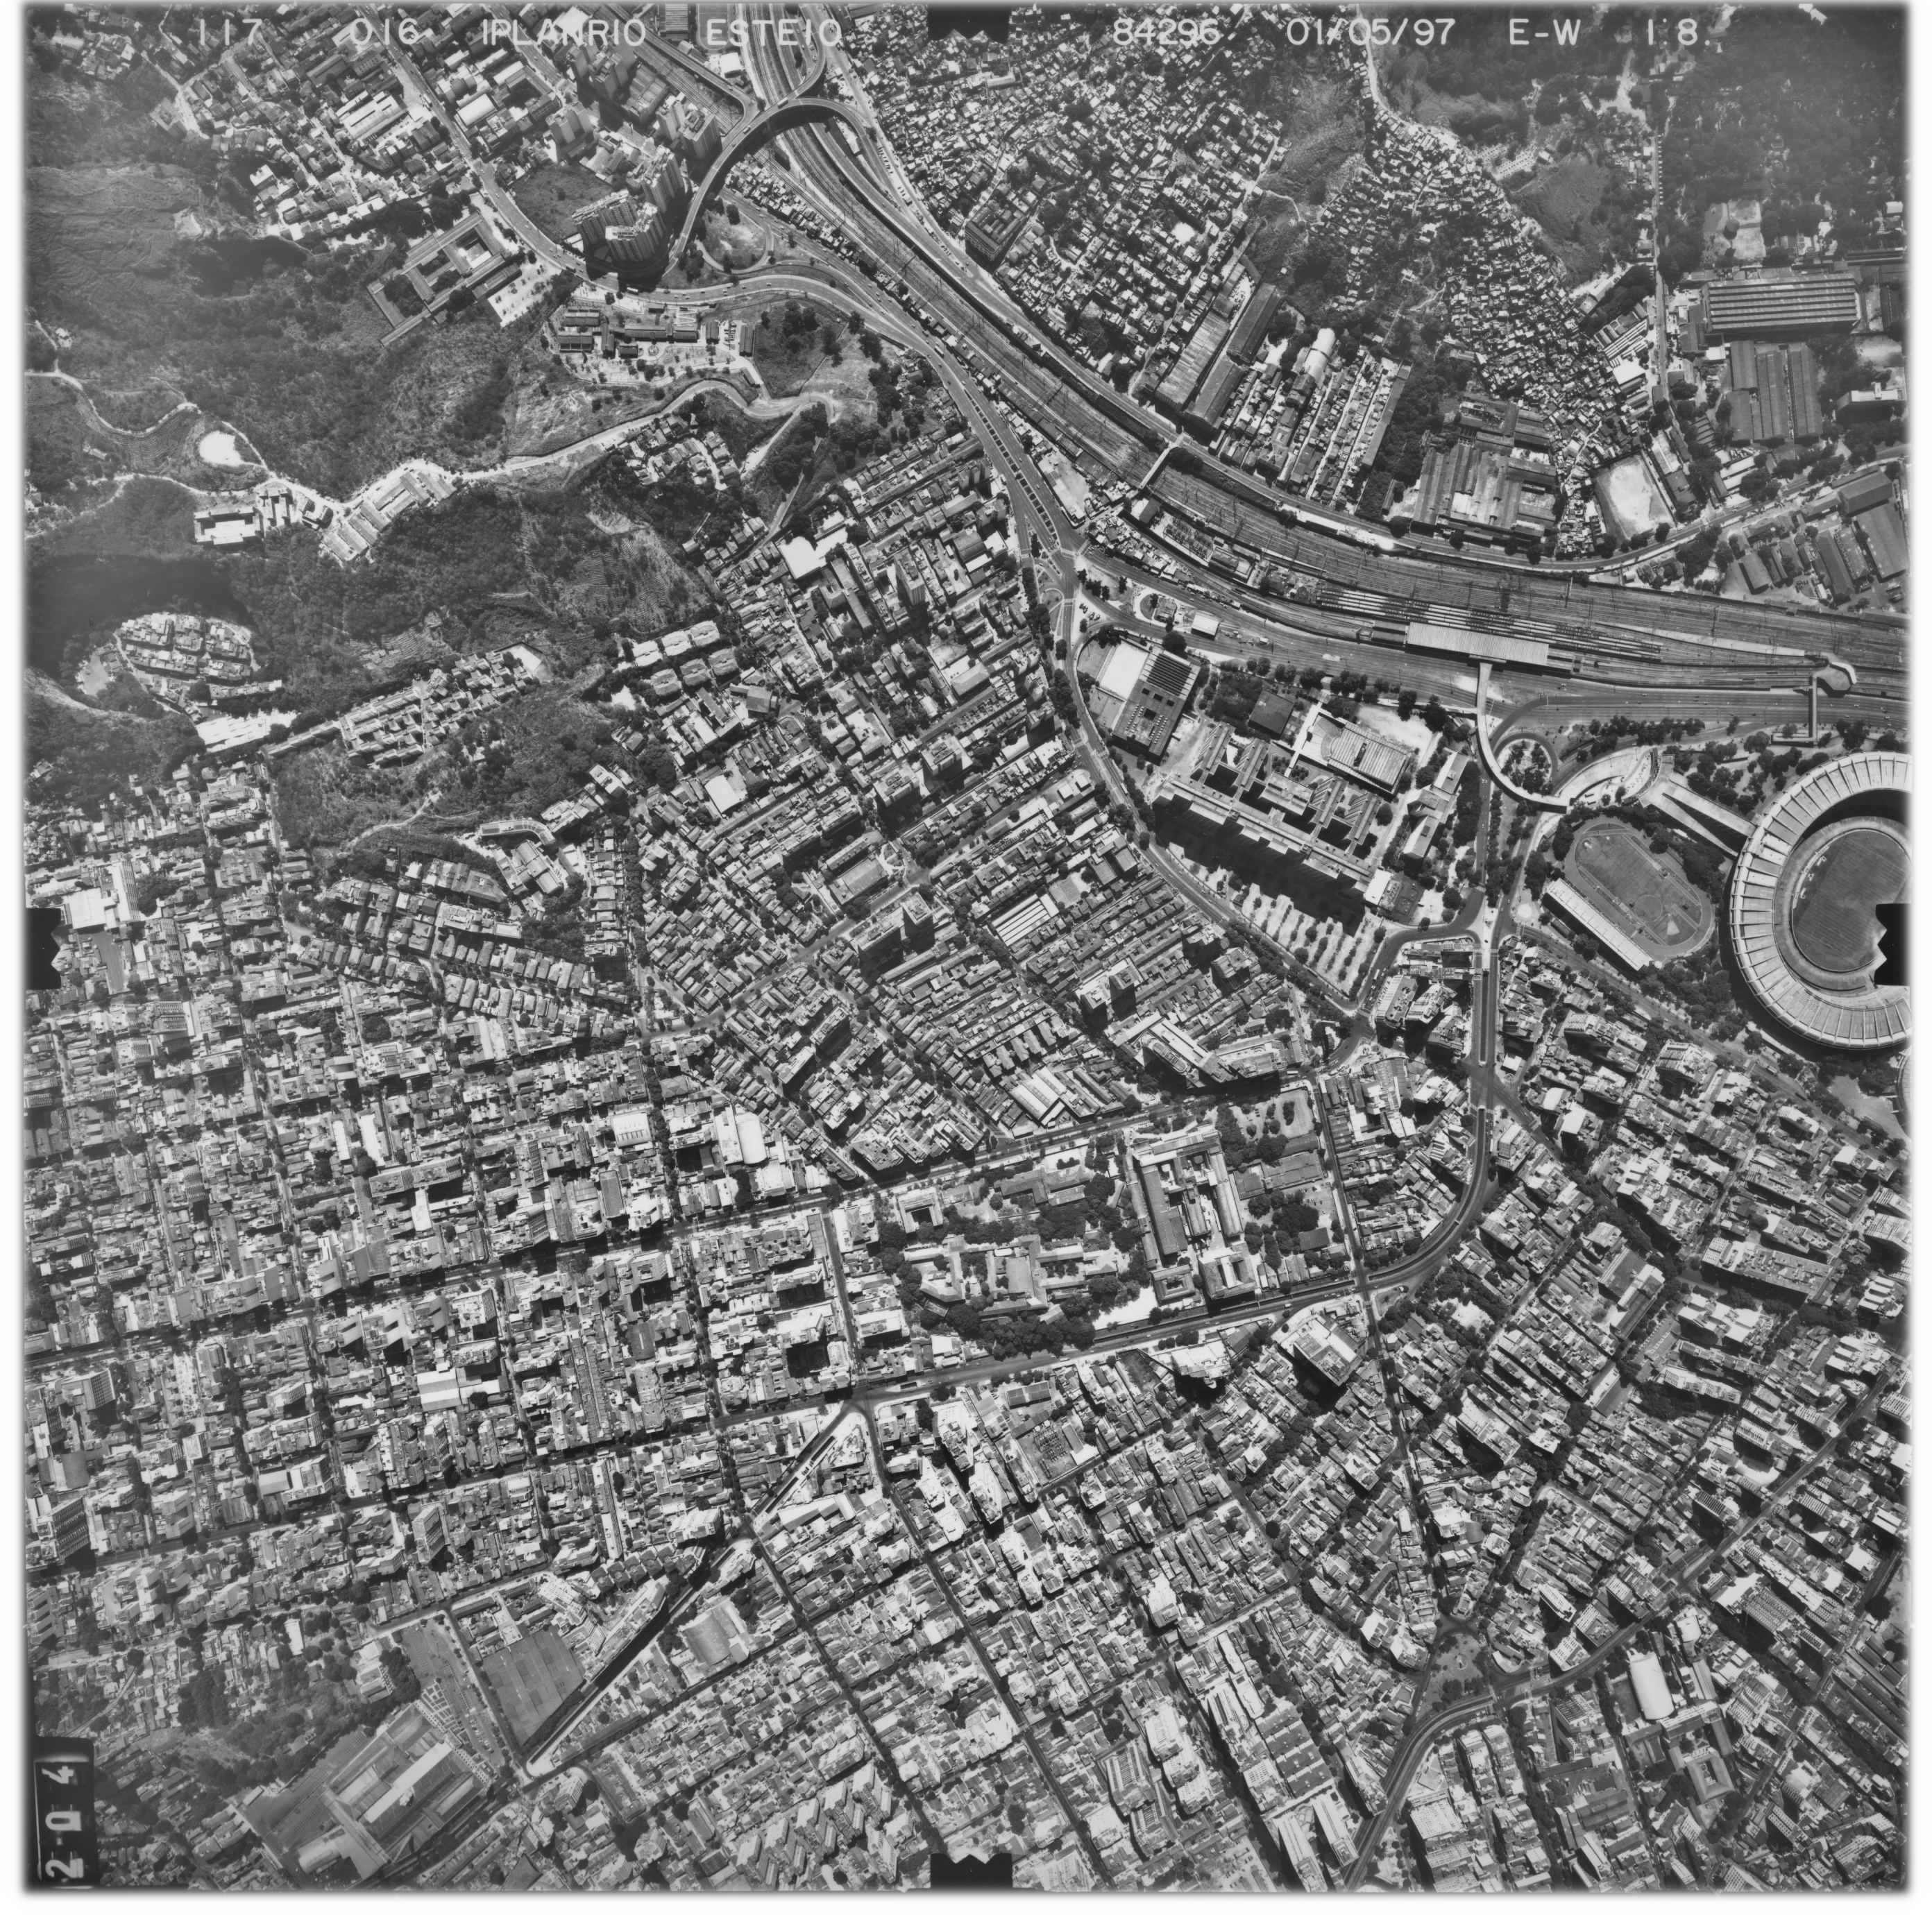
\includegraphics[width=0.3\hsize]{figuras/1997_016_300dpi.png}}}\hfill
  \subfloat[][]{\label{17}
    \setlength{\fboxsep}{0pt}
    \fbox{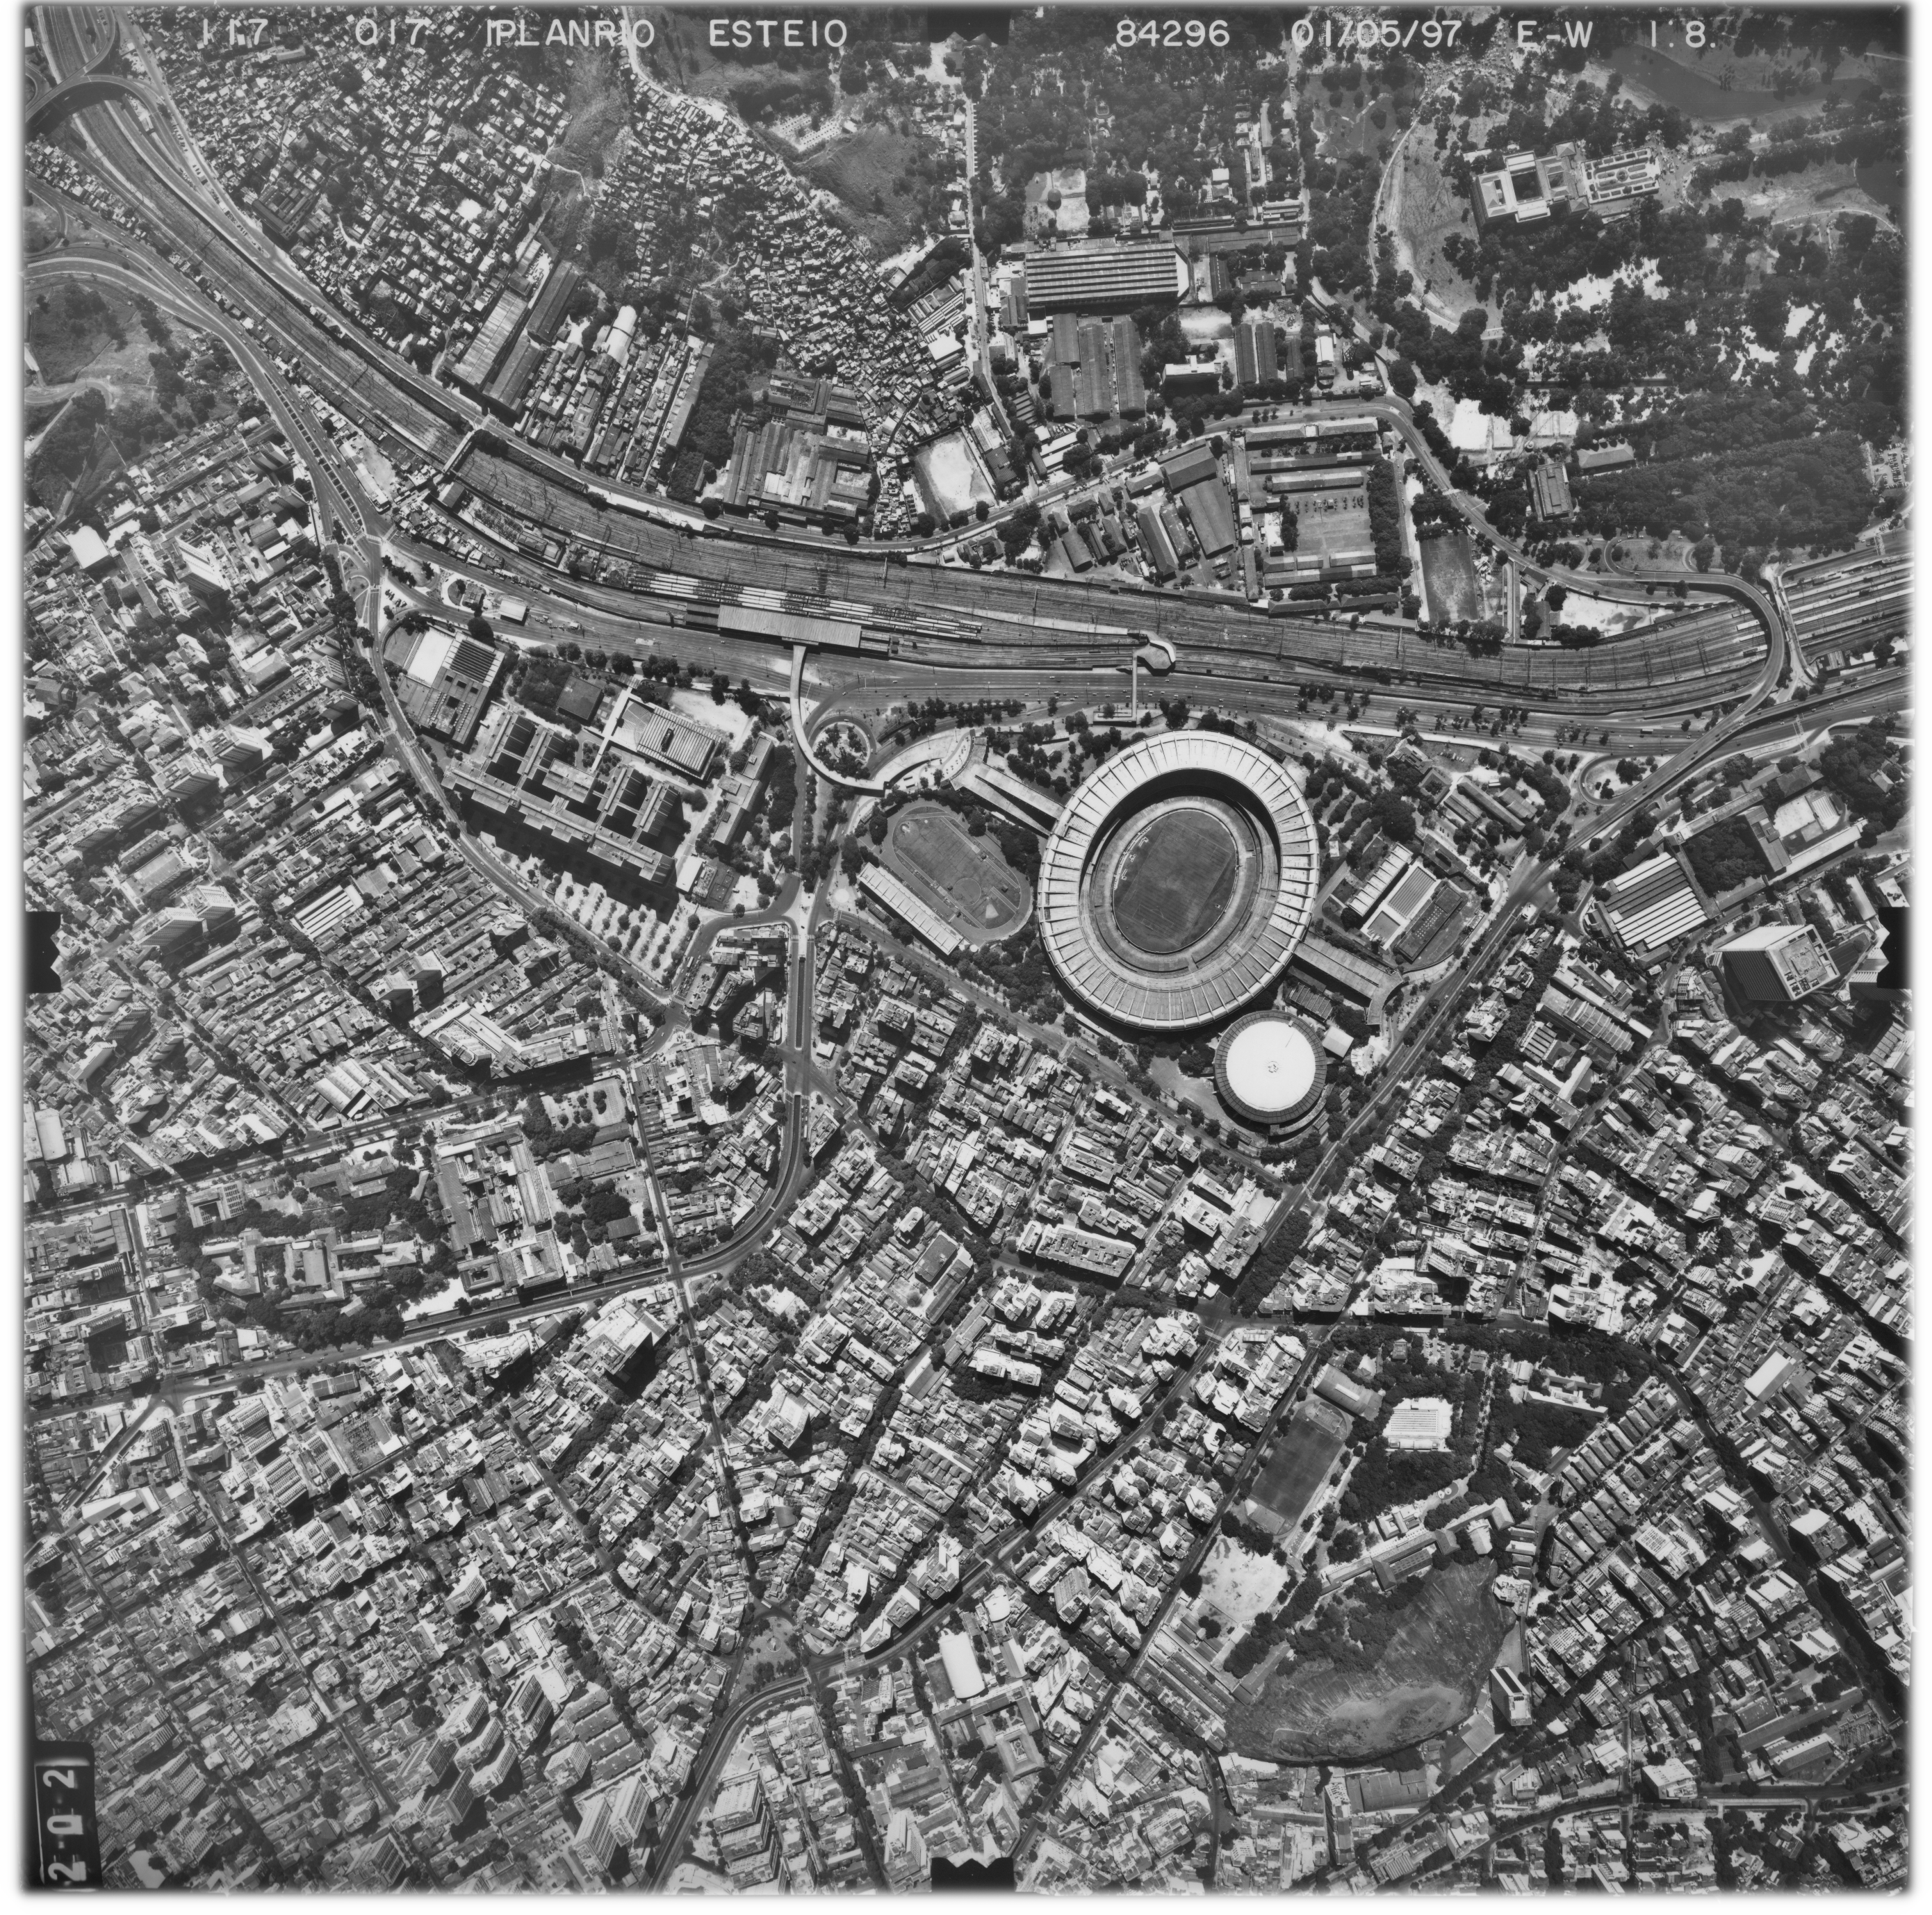
\includegraphics[width=0.3\hsize]{figuras/1997_017_300dpi.png}}}\hfill
  \subfloat[][]{\label{18}
    \setlength{\fboxsep}{0pt}
    \fbox{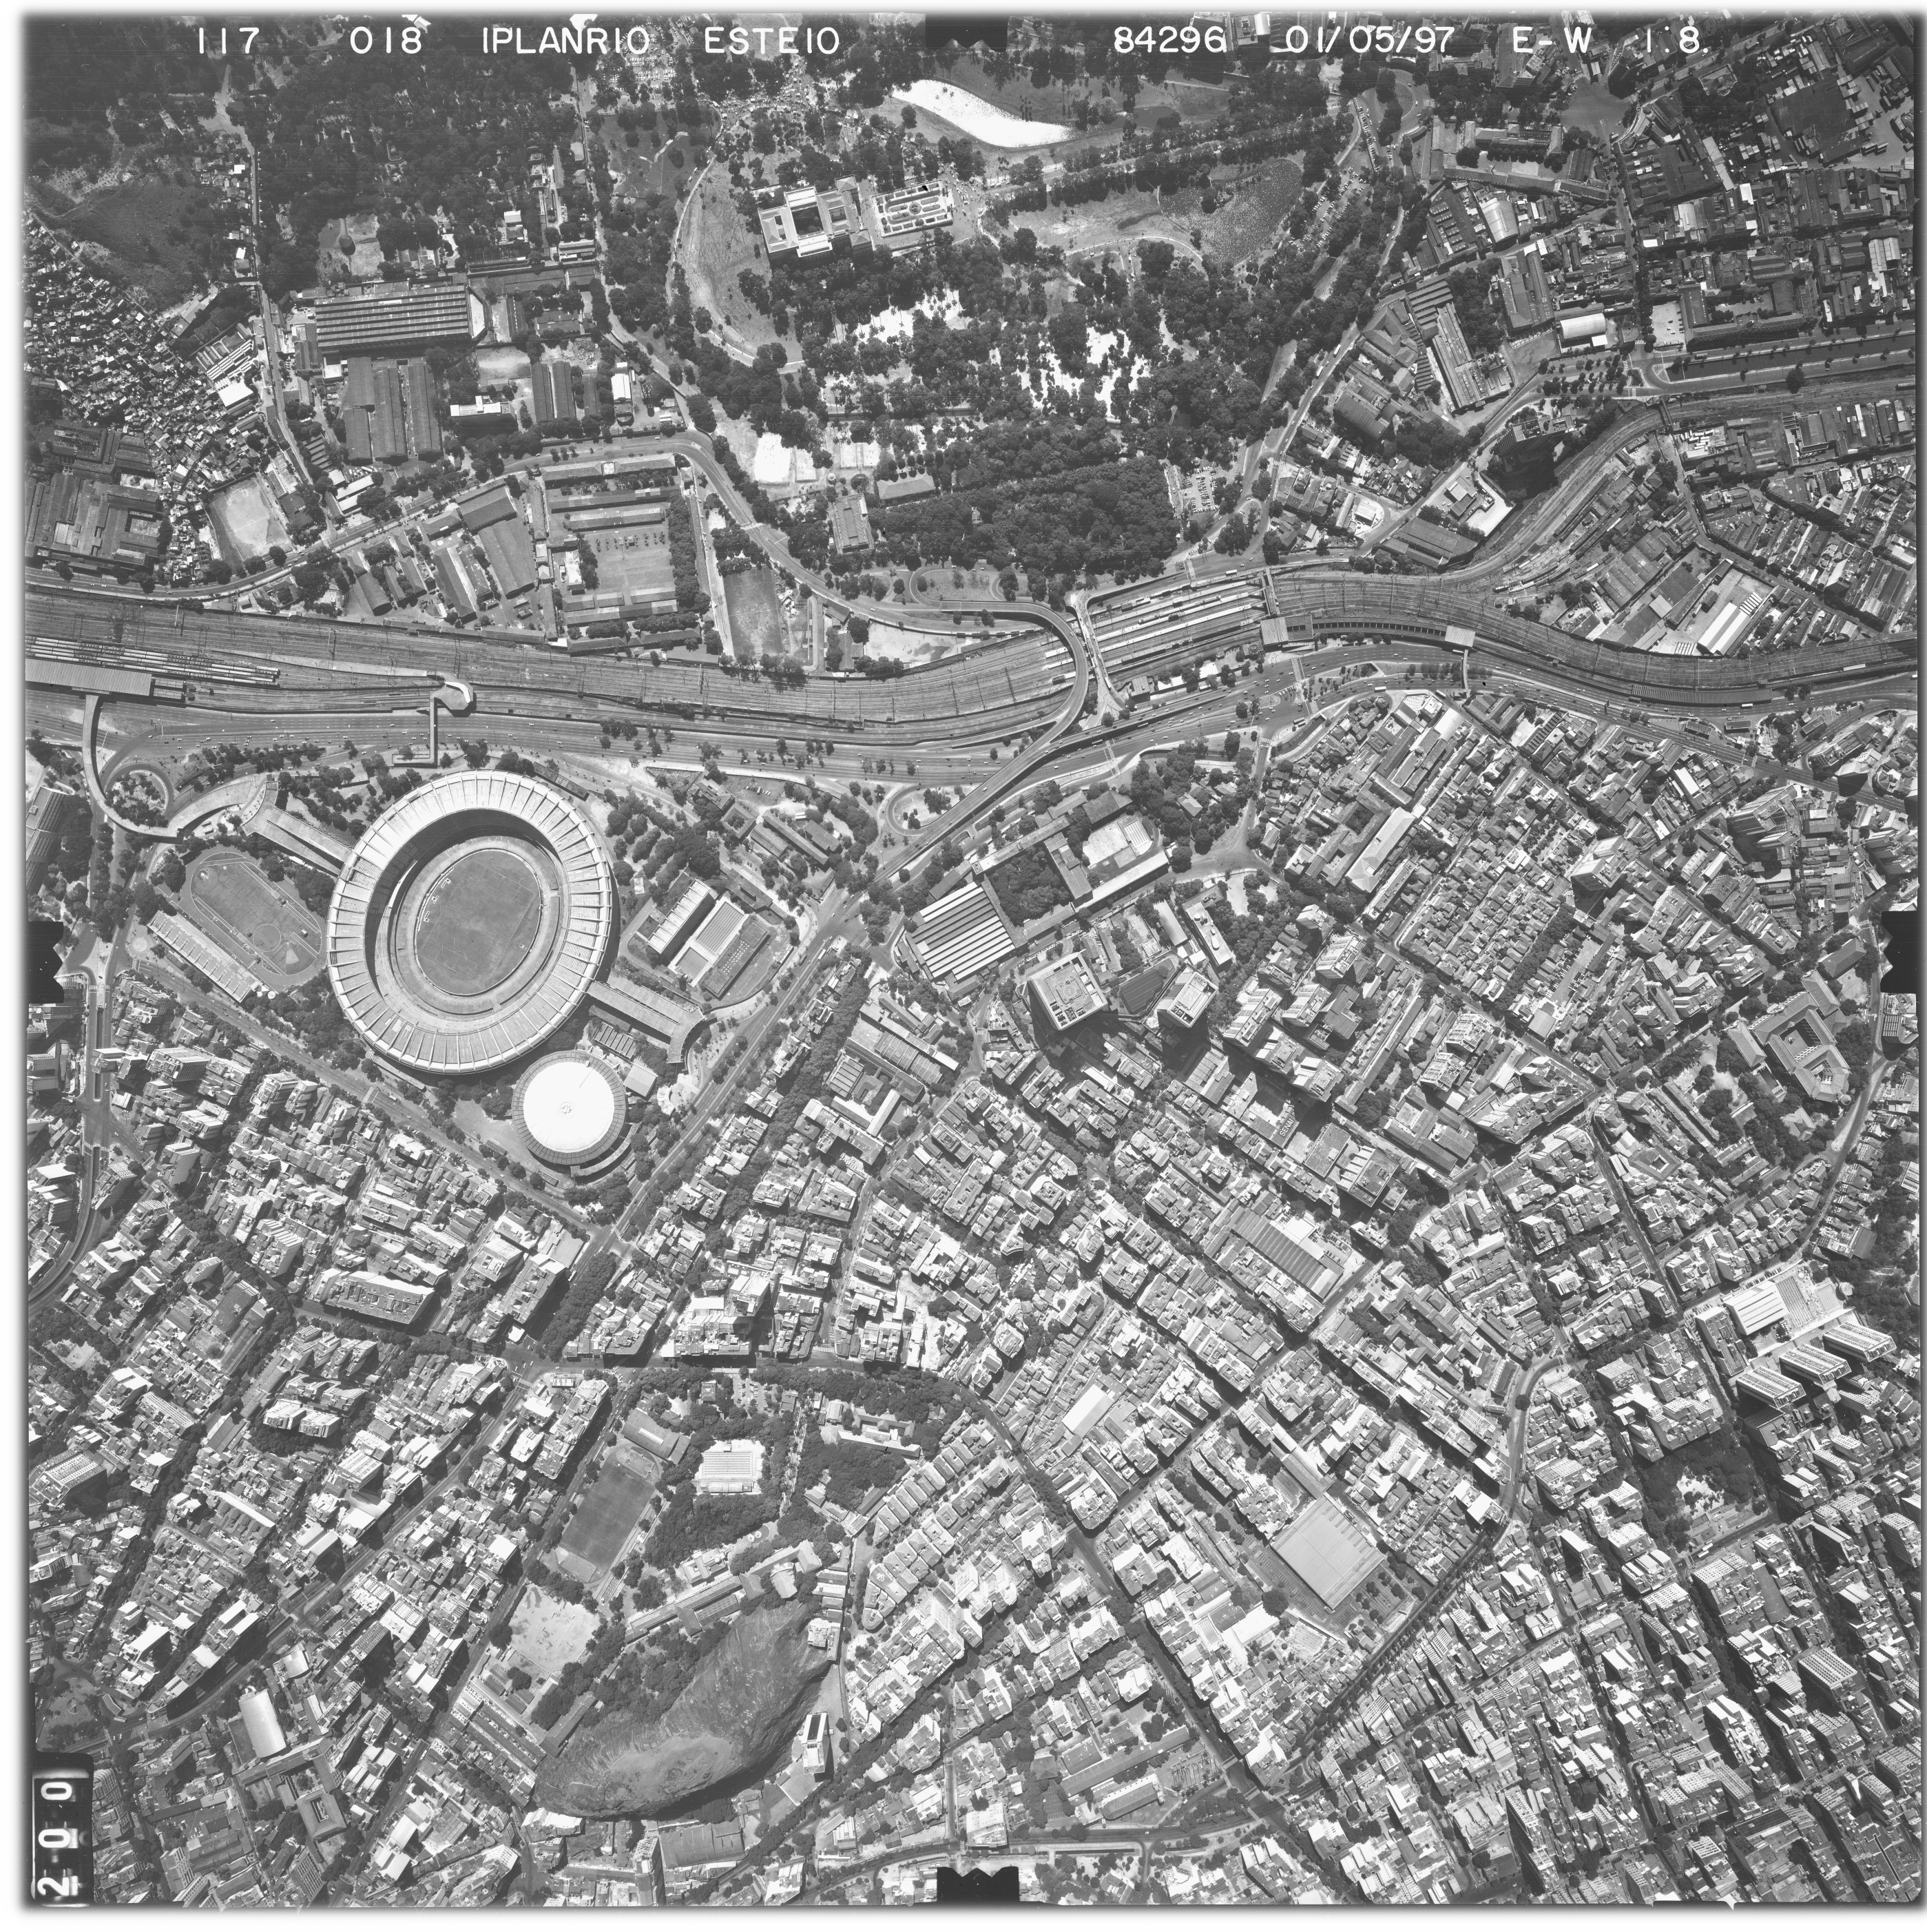
\includegraphics[width=0.3\hsize]{figuras/1997_018_300dpi.png}}}
  \legend{\subref{16} 16;
          \subref{17} 17; e
          \subref{18} 18}
  \source{Arquivo do Projeto E-Foto sobrevoo UERJ de 1997.}
\end{figure}

Um conjunto de imagens de exemplo do e-foto\footnote{O conjunto de imagens pode ser obtido em \url{http://www.efoto.eng.uerj.br/download/imagens-e-dados}}, conforme observado na Figura \ref{16_17_18}, foi adotado nos testes principais deste trabalho. Por simplicidade, estas imagens de sobrevoo da região da Tijuca, com foco na área da UERJ, realizado em 1997 e cedido ao LFSR pelo IPP, serão denominadas 16, 17 e 18 quando exibidas no Capitulo \ref{results}.


\section{Definição dos critérios de análise das opções disponíveis}

Com a fase de estudos finalizada, fez-se indispensável a definição de critérios para comparação entre os métodos disponíveis, tanto para detectar e descrever feições, quanto para compará-las e restringir o conjunto com uma análise geométrica. Estes critérios devem permitir o entendimento de suas diferenças, quantitativas e qualitativas, e como eles se comportariam para imagens de relevância fotogramétrica. Adotaram-se então 4 critérios de análise:

\begin{itemize}
    \item Tempo de execução e memória alocada
    \item Distribuição e volume das respostas
    \item Verificação da qualidade
    \item Viabilidade de filtragem dos melhores pontos
\end{itemize}


\subsection{Tempo de execução e memória alocada}

Para análise do tempo de execução foram isolados pontos específicos dos códigos testados e em desenvolvimento com a biblioteca ``Chrono'', que é parte das bibliotecas nativas do C++11, e adotado retorno de intervalos em milissegundos (ms). Para a quantificação de memória alocada foram feitas macros de cálculo do espaço reservado para as principais estruturas em uso em cada código analisado. Entende-se que a escolha de pontos específicos do processamento, bem como de algumas estruturas principais, não reflete o total de tempo e memória usados. Contudo, é razoável esperar que seja possível averiguar, pela diferença entre as somas obtidas e um contador externo ao programa (como a função \textit{time -v $<$program$>$} do sistema Linux), se as partes selecionadas são realmente as mais significativas de todo o processo.


\subsection{Distribuição e volume das respostas} \label{Dist_gruber}

Este critério implica na percepção visual do preenchimento da região de sobreposição das imagem com pontos correlatos que puderam permanecer até o fim do processo, assim se tornando pontos de costura, bem como do decaimento do número de pontos chaves e de correlações após as etapas de refinamento como a verificação geométrica. Para análise e avaliação da distribuição de respostas será utilizado o conceito de regiões de gruber \cite{manual_photogrammetry}. Tal conceito afirma que apenas quando temos pontos bem distribuídos e de preferência cobrindo distintas regiões de interesse na área de sobreposição das imagens, conforme a ilustra a Figura \ref{gruberarea}, podemos ter uma solução robusta e que elimine a paralaxe vertical.


\begin{figure}[!ht]{12cm}
  \caption{Regiões de interesse para distribuição de pontos de gruber} \label{gruberarea}
  \includegraphics[width=\hsize]{figuras/gruberarea.png}
  %\legend{Texto da legenda.}
  \source{Imagem adaptada de \citeauthoronline{manual_photogrammetry} (\citeyear{manual_photogrammetry})}
\end{figure}
%Para a analise da distribuição de respostas será utilizado o conceito de pontos de gruber 

\subsection{Verificação da qualidade}

Para este critério de análise podem ser considerados tanto a analise visual dos pontos medidos após sua carga no módulo de aerotriangulação ou numa imagem do par, quanto o valor numérico de erro quando usamos uma transformação projetiva (homografia) para projetar pontos de uma imagem sobre a outra na qual há correlatos previamente estimados. 

\subsection{Viabilidade de filtragem de melhores pontos}

A viabilidade de filtragem dos melhores pontos serve ao princípio de não sobrecarregar o projeto com pontos. Logo, é importante que parâmetros adicionais possam ser adotados na solução final para efetuar controle do total de pontos gerados.



\section{Planejamento de testes comparativos}

Para verificar a viabilidade de execução de todos os algoritmos selecionados foram localizadas bases comuns de código, principalmente entre os exemplos do módulo \textit{features2d}\footnote{Materiais disponíveis em \url{https://docs.opencv.org/4.5.4/d9/d97/tutorial_table_of_content_features2d.html}}. 
Os exemplos para estudo deste módulo incluem a produção e uso de detectores, bem como a apresentação de diferentes extratores de feições, métodos de correlação e a verificação geométrica, incluindo a aplicação na localização de objetos em imagens e de rastreamento em vídeo.
Foram então planejados e efetuados testes de configuração com os diferentes algoritmos em estudo adotando-se um mesmo fluxo de base. Foram incorporadas e testadas diferentes técnicas de tomada de medidas para extrair os valores que atendessem aos critérios definidos. Ao fim deste planejamento, foi possível esboçar um conjunto de variações nas entradas que pudessem ser usadas para testar o produto final.



\section{Codificação da solução}

Tendo feito modificações e testes de uso de diversos exemplos de código da biblioteca, iniciou-se a fase de codificação de um produto final (disponível no Apêndice \ref{codigofonte}) integrando aspectos estudados para atender o objetivo deste projeto. Por simplificação foi adotada a interface de linha de comandos, entendendo que esta poderá ser acessada diretamente por outro software, como o e-foto, para obter os pontos de costura dado um conjunto de argumentos variado.

\begin{figure}[!h]{15cm}
  \caption{Fases da execução da solução de linha de comando proposta} \label{macro}
  \includegraphics[width=\hsize]{figuras/macro.png}
  %\legend{}
  \source{O autor}
\end{figure}

De um ponto de vista geral, as partes do processo podem ser descritas como indica a Figura \ref{macro}, onde é observado que além do processamento principal é  a necessidade de ao menos duas fases dedicadas à interface com o mundo externo. A interpretação dos argumentos lida com informações de entrada que configuram o pedido de processamento. A persistência de resultados lida com a saída das respostas encontradas durante o processo principal. Ao seu tempo, o processo principal pode ser subdividido em 3 outros focados em tratamento das imagens individualmente, dos pares sugeridos pelo usuário e das medidas identificadas pelo processamento de pares.

Por sua vez, as tentativas de acomodar a solução com programação procedural apenas, como transcorre na maioria dos exemplos de OpenCV, mostrou-se de grande complexidade para a documentação, pois muitas em alguns pontos o código tornava-se de difícil leitura. Por exemplo, assumindo que uma função \textit{knnMatch} pode retornar os $n$ vizinhos mais próximos de cada um dos $m$ pontos chaves descritos, e que este processo seria repetido $p$ vezes para atender aos pares processados, 
teríamos um vetor com 3 dimensões causando uma complexa administração de índices ao acessar tais informações, ou seja, algo como \textit{knnResult[i][j][k]} seria necessário para indicar o k-ésimo vizinho do j-ésimo ponto chave da primeira imagem do i-ésimo par de imagens.

\begin{figure}[!h]{16cm}
  \caption{Diagrama de classe da solução} \label{classdiagram}
  \includegraphics[width=\hsize]{figuras/classdiagram.png}
  %\legend{}
  \source{O autor}
\end{figure}

Pela adoção de um modelo de programação orientado à objetos podemos ainda expressar a estrutura da solução proposta em termos de linguagem gráfica na notação UML, conforme ilustra a Figura \ref{classdiagram}. No diagrama de classes um controlador de processo define métodos para as principais atividades, além de um método de impressão dos argumentos para uso da solução. O controlador de processo acomoda todas as imagens carregadas através do arquivo de entrada, instancia os pares cuidando das ligações necessárias com suas imagens (evitando assim a repetição das informações de imagens em memória) e cria, atualiza ou junta pontos durante o processamento de medidas (haja visto que pontos de costura precisam ser medidos em diferentes imagens). No processamento de pares e imagens, o controlador repete a chamada de métodos apropriados de cada imagem a ser descrita ou par a ser correlacionado. 

Objetos de OpenCV que configuram pontos chaves e correlações, bem como matrizes de descrição ou transformações geométricas, são apresentados no diagrama de classe e cabe notar que a OpenCV usa índices numéricos (ligações indiretas) que apontam estes objetos pela posição em que se encontram num \textit{container} de dados, tipicamente vetores da biblioteca padrão de C++, a STL (acrônimo para \textit{Standard Template Library} ou biblioteca de modelos padrão). 

A ligação entre as classes imagem e ponto faz-se importante em dois momentos e nos dois sentidos, sendo caracterizada a ligação com o ponto, isto é, partindo da imagem, como prioritária. Isto se justifica pelo algoritmo de integração da medidas dos pontos de costura quando estes ocorrem em pares distintos. Nos casos onde uma imagem participa de diversos pares é necessária a busca na imagem pela medida, a fim de determinar se esta já foi registrada durante o processamento de outros pares com a mesma imagem. Ao seu tempo, a ligação com a imagem, partindo do ponto, faz-se necessária em termos de entrega do produto final, na qual cada medida do ponto em distintas imagens deve ser corretamente associada. A associação das medidas de cada ponto podem então ser atendidas com uma simples cópia do índice da imagem, sem que isso implique em perda de performance ou grande consumo de memória.



\subsection{Escolha de argumentos}

Para possibilitar alguma flexibilidade de uso, a solução final requer que sejam apontados nomes de arquivos de entrada e sugeridos outros dois nomes para os arquivos de saída. Além destes arquivos, é possível adicionar opções de configuração que podem, entre outras coisas, trocar o método de detecção e descrição em uso, alternar entre os métodos de correlação disponíveis e inserir critérios para limitar o conjunto de resultados obtidos.

O primeiro dos arquivos de entrada esperados é uma lista de caminhos para as imagens que serão processadas, precedidas de seus índices no projeto, pois o resultado será apresentado em termos destes índices de imagens. O segundo arquivo deve indicar quais pares de imagens devem ser processados. Neste segundo arquivo, apenas os índices de imagens precisam ser apresentados.

Alternativamente, uma opção \textit{mode} pode ser usada para escolher processar todos os pares possíveis (\textit{ALL}) ou através da sequência (\textit{SEQUENCE}), na qual as imagens foram descritas. Deste modo, se \textit{SEQUENCE} está ativo e as imagens listadas são 16, 17 e 18, por exemplo, os pares serão 16 com 17 e 17 com 18.

Já os nomes dos arquivos de saída devem ser indicados para que sejam gravados, no primeiro arquivo, as medidas nas imagens para cada ponto de costura, e no segundo arquivo, o índice e tipo de cada ponto. Neste segundo arquivo são gravados então o tipo \textit{Photogrammetric}, que indicam para o e-foto que estes podem ser usados na aerotriangulação, e uma sequência com 6 zeros (valores para E, N, H e suas precisões destas 3 medidas, quando disponíveis). A gravação com zeros é feita para que o e-foto não precise de quaisquer alterações evitando assim erros de leitura. Cabe notar que no processo de aerotriangulação as coordenadas de mundo destes pontos serão sobrescritas.

Na versão 472\footnote{Método disponível em \url{https://sourceforge.net/p/e-foto/code/472/tree/trunk/qt/interface/ProjectUserInterface\_Qt.cpp\#l2635}} do código do e-foto, observou-se que o método \textit{importPointsFromTxt2} pode ser acessado somente pelo atalho de teclado (``Ctrl+Shift+P''). Este está disponível durante a execução do módulo de projetos e resulta no pedido de dois arquivos a saber: arquivo de coordenadas ENH (nossa segunda saída); e o arquivo de medidas no espaço das imagens.

Argumentos extras para o processamento incluem:

\begin{itemize}
    \item \textbf{detector} para selecionar o algoritmo adotado (AKAZE, ORB, SIFT ou SURF);
    \item \textbf{ccheck} para acionar a verificação cruzada de correlações com BFM (desligando o FLANN);
    \item \textbf{verbose} para ligar a impressão de informações do processamento úteis na confecção dos resultados apresentados no Capítulo \ref{results};
    \item \textbf{number\_f} para definir o número $f$ de pontos chaves o algoritmo ORB irá detectar;
    \item \textbf{force\_f} para ativar a limitação de detecções nos demais algoritmos baseado em $f$;
    \item \textbf{gruber\_roi} para ativar a limitação da área passível a detecção de pontos chave;
    \item \textbf{help} para exibir os parâmetros e suas descrições;
    \item \textbf{init\_index} para definir o identificador inicial dos pontos de costura;
    \item \textbf{list\_pairs} para registrar os pares que possuem solução com uma taxa de \textit{inliers} desejada;
    \item \textbf{limit\_out} para limitar a saída de pontos de costura por par;
    \item \textbf{mode} para definição do modo em que serão selecionados os pares;
    \item \textbf{n\_measures} para limitar os pontos àqueles contidos em um mínimo de $n$ imagens;
    \item \textbf{residue} para definir o valor máximo do resíduo aceito na verificação geométrica;
    \item \textbf{scale} para definir o denominador para realizar a redução das imagens;
\end{itemize}

A impressão de toda a lista de argumentos foi programada para atender a opção \textit{help}, ou no caso de quaisquer falhas de execução do processo que inviabilizem a gravação de resultados. Erros graves que podem suspender o processamento geram mensagens ao usuário, como a inviabilidade de abrir uma das imagens indicadas pelo usuário, enquanto que falhas toleráveis, como a inviabilidade de obter medidas para um par, são contornadas e podem ser reportadas ao final do processo.



\subsection{Processamento de imagens}

No processamento de imagens se cumprem as extrações dos pontos chaves do conjunto de imagens. Há método em OpenCV para fazê-lo para um conjunto de imagens pré-carregadas pelo usuário, contudo entende-se que se o tamanho de todas as imagens for muito grande pode ser inviável usar este recurso. Logo, como indicado na Figura \ref{fl:imagens}, adotou-se uma sequência de atividades onde cada imagem é aberta, tem suas informações extraídas e então fechada, tendo o número de pontos-chave relatado se solicitado. 

\begin{figure}[!h]{15cm}
  \caption{Diagrama de atividades para o processamento de imagens} \label{fl:imagens}
  \includegraphics[width=\hsize]{figuras/Fluxo_Imagem.png}
  %\legend{}
  \source{O autor}
\end{figure}

De igual modo, os exemplos disponibilizados pela OpenCV demonstram a detecção e descrição simultaneamente, porém optamos por separar essas atividades para que uma melhor compreensão dos algoritmos possa ser alcançada. Isto ajuda na quantificação de tempos individuais para estas etapas e poderia ser usado para mesclar os métodos ou adotar algoritmos especializados em uma das duas atividades. Medidas de tamanho das estruturas podem demonstrar como o processo escala em memória e ajudam a compreender qual a quantidade de memória que pode vir a ser necessária para grandes conjuntos de imagens com cada método.



\subsection{Processamento de pares}

O processamento de pares faz correlação de pontos chaves descritos previamente para as imagens e, em seguida, verifica se é possível obter uma solução de transformação geométrica entre o conjunto de pares, considerando um erro máximo de reprojeção aceitável. Estas atividades são implementadas integralmente pela OpenCV, mas é importante realizarmos atividades extras, como as ilustradas na Figura \ref{fl:pares}, para selecionar melhores correlações e registrar os erros de medida observados. Estes erros são possíveis de computar usando a transformação geométrica, que restringe os pontos da solução final.

\begin{figure}[!h]{15cm}
  \caption{Diagrama de atividades para o processamento de pares} \label{fl:pares}
  \includegraphics[width=\hsize]{figuras/fluxo_pares.png}
  %\legend{}
  \source{O autor}
\end{figure}

A correlação dos pontos chaves pode ser feita por força bruta (BFMatcher na OpenCV), isto é, cada ponto chave em uma imagem é confrontado com todos os pontos chaves da outra imagem no par. Deste modo, são preservadas as menores distâncias no espaço de descrição observadas para cada ponto chave processado. Embora caro computacionalmente, ficando seu uso restrito aos pequenos conjuntos de dados, este processo permite a verificação cruzada de vizinhos mais próximos. Isto equivale a responder a questão ``se um ponto chave $P$, na primeira imagem, possui melhor correlação com um ponto chave $Q$, na segunda imagem, a análise no sentido oposto também é verdadeira?'', onde o ``afirmativo'' corresponde a correlação cruzada.

A alternativa viável ao processamento de correlações por força bruta, quando o conjunto de pontos chaves é muito grande, é a busca por vizinhos mais próximos aproximados (FlannBasedMatcher na OpenCV). Ela usa estruturas especializadas para a busca espacial, como as árvores de k-dimensões (KD-Tree) ou o hash sensível à localidade (LSH), implementadas e amplamente divulgadas pela biblioteca flann\footnote{\textit{Fast Library for Approximate Nearest Neighbors} está disponível em \url{https://github.com/flann-lib/flann}}. Neste caso, a estrutura de busca espacial deve estar alinhada ao descritor usado, ou seja, descritores binários requerem algoritmos de hash, enquanto descritores modelados com números reais, como SIFT e SURF, usam KD-Tree. Esta diferença é notável na própria forma de computar distâncias, pois a distância aplicável aos descritores binários é a distância de Hamming \cite{ORB}.

O ganho em tempo de execução quando utilizados vizinhos mais próximos aproximados é contraposto pela inviabilidade de verificação cruzada. Contudo, um outro critério de eliminação pode ser adotado ao observar a razão entre a distância para o vizinho mais próximo de um ponto chave e o segundo vizinho mais próximo. A lógica embarcada nesta observação é que um ponto chave com apenas um vizinho mais próximo é potencialmente mais relevante do que aqueles que possuem mais de um vizinho em seu entorno \cite{SIFT2004}.

É importante notar que apenas selecionar as melhores correlações pode não ser suficiente para eliminar erros grosseiros. Logo, uma segunda rodada de análise, considerando as restrições geométricas que podem ser observadas para imagens de uma mesma cena, deve ser aplicada. Nesta atividade, um outro módulo de OpenCV, \textit{calib3d}, apresenta contribuições importantes, das quais adotamos o método \textit{findHomography}. Sua aplicação principal é o cálculo de uma transformação projetiva entre os planos das imagens dadas por um conjunto de pontos correlatos. Aqui aplicam-se as técnicas de ajustamento robustas discutidas anteriormente e, como consequência, podem ser identificados e removidos quaisquer pares de pontos chaves que apresentem erro de reprojeção superior a algum limiar definido pelo usuário.

De posse da transformação geométrica podemos ainda registrar e classificar as correlações restantes segundo o resíduo observado. Entendemos que este pode ser um critério melhor do que a distância de correlação propriamente quando se trata da seleção dos melhores pontos de costura para um bloco de imagens.



\subsection{Processamento de medidas}

Com os dados obtidos após o processamento de pares, resta a organização das medidas a serem salvas como resultado do processo. Isto é feito pelo próprio controlador de processo, tendo em vista que ele é o detentor de todas as informações e que os pontos de costura individualmente não devem realizar qualquer processamento, além do registro de suas medidas, evitando indexar a mesma imagem mais de uma vez. 

Embora seja viável na OpenCV correlacionar feições de uma imagem com diversas outras em apenas uma chamada, algo que se aplica muito bem para aplicações de detecção de objetos, esta abordagem parece inapropriada para a finalidade de costura de blocos fotogramétricos, pois tornar-se-ia complexo distinguir entre padrões repetitivos de bons pontos de costura observáveis em mais de duas imagens. Porém, para o e-foto e para a fotogrametria em geral, uma faixa de aerofotos pode ter inúmeras imagens, todas com sobreposição regular e muitas faixas, onde a sobreposição é menor, mas pode haver boas feições. Logo, é desejável a percepção de pontos em 3 ou mais imagens, mesmo se considerarmos apenas uma faixa com recobrimento lateral de aproximadamente 60\%, que é o caso da maioria das faixas de sobrevoo convencionais. Para mais, aerolevantamentos com drones podem ter ainda mais sobreposição para compensar os pequenos formatos de sensores e a falta de estabilidade destas plataformas. 

Logo, julgamos que não cabe registrar todos os pares de pontos correlatos diretamente sem antes efetuar qualquer crítica sobre a possibilidade de um mesmo ponto chave ser bem correlacionado, e com pouco resíduo, em diferentes pares de imagens. O que se espera obter é a observação de uma propriedade transitiva que afirma, ``Se $a=b$ e $b=c$, então $a=c$'', ou seja, pela correlação ter sido realizada em imagens par-a-par, um mesmo ponto pode estar em dois ou mais pares e ter algumas de suas coordenadas ligadas a duas outras imagens ou mais. Uma extensão da mesma propriedade pode ser importante para lidar com o encadeamento não sequencial de pares, isto é, ``Se $a=b$, $c=d$ e posteriormente é constatado que $b=c$, então $a=c$, $a=d$ e $b=d$''.

\begin{figure}[!h]{15cm}
  \caption{Diagrama de atividades para o processamento de medidas} \label{fl:medidas}
  \includegraphics[width=\hsize]{figuras/fluxo_medidas.png}
  %\legend{}
  \source{O autor}
\end{figure}

Com o entendimento destas possibilidades de combinação de pares podemos formular um diagrama de atividades que incorpore a criação, atualização e fusão de pontos chaves, como o ilustrado na Figura \ref{fl:medidas}. Então para todos os \textit{inliers} de cada par repete-se o processo de registro das medidas observadas. A criação de um novo ponto de costura ocorre sempre que nenhuma das imagens do par registrou previamente a medida observada. Se apenas uma delas registrou o previamente a medida observada, então existe um ponto de costura a ser atualizado pela adição de mais uma medida. Contudo, se ambas as imagens de um par já registraram as medidas observadas, pode haver dois pontos de costura distintos que se aplicam a uma mesma feição do espaço objeto. Neste caso, as medidas devem ser mescladas num único pontos de costura. 

Para a busca na imagem por medida pré-existente adotou-se a estrutura de dados \textit{map}\footnote{Ajustes necessários para uso desta estrutura com os pontos do OpenCV foram indicados em \url{https://stackoverflow.com/questions/26483306/stdmap-with-cvpoint-as-key}} da STL, pois esta possui tempo de acesso reduzido, aplicando internamente o algoritmo de busca binária. Outras alternativas seriam adotar uma \textit{KD-tree}, com tempo de acesso equivalente ao \textit{map}, ou um algoritmo de \textit{hash} (como implementado em \textit{unordered\_map}) com tempo de resposta menor, mas possivelmente com elevado custo de armazenamento.


\subsection{Persistência de dados}

A persistência de dados será realizada sob os formatos de arquivos adotados pelo método de inserção pré-existente no e-foto. O primeiro arquivo solicitado pelo e-foto identifica o ponto, atribui um tipo e apresenta os valores para E, N e H e as precisões deste no espaço objeto. Assim, para cada ponto de costura gerado teremos uma linha, como pode ser observado na Figura \ref{exemp_ENH}, onde o primeiro valor equivale à identificação do ponto seguido pelo tipo de ponto. Os demais valores são zerados, pois não se aplicam aos pontos fotogramétricos. 

\begin{figure}[!ht]{12cm}
  \caption{Exemplo do arquivo de persistência de pontos.} \label{exemp_ENH}
  \fbox{\includegraphics[width=\hsize]{figuras/exemplo_ENH.png}}
  \legend{Da esquerda para a direita as colunas representam: identificação de cada ponto; tipo de ponto; E; N; H; e suas respectivas precisões.}
  \source{O autor.}
\end{figure}

\begin{figure}[!ht]{12cm}
  \caption{Exemplo do arquivo de persistência de medidas.} \label{Exemp_saida}
  \subfloat[][]{\label{saida1}
    \fbox{\includegraphics[width=0.45\hsize]{figuras/exemplo_saida1.png}}}\hfill
  \subfloat[][]{\label{saida2}
    \fbox{\includegraphics[width=0.45\hsize]{figuras/exemplo_saida.png}}}\\
  \legend{Da esquerda para a direita as colunas representam: índice na imagem; índice do ponto; coluna; e linha de medição do ponto na imagem.\\
  \subref{saida1} Medidas dos pontos de índice 462 à 466; e\\
  \subref{saida2} Medidas dos pontos de índice 467 à 470.}
  \source{O autor.}
\end{figure}

Por sua vez, a Figura \ref{Exemp_saida} ilustra o conteúdo do segundo arquivo solicitado, no mesmo processo de importação de pontos fotogramétricos pelo e-foto. Este arquivo leva as medidas dos pontos em coordenadas digitais (no espaço imagem) a serem inseridas. Quatro colunas são usadas para: a identificação da imagem na qual o ponto foi medido; indexar do ponto medido; e transmitir as coordenadas em coluna e linha, respectivamente. 

Cabe destacar que a carga de pontos fotogramétricos no e-foto poderia ainda ser modificada para eliminar a necessidade do arquivo que identifica o ponto, pois este não agrega qualquer informação que não possa ser derivada do segundo formato de arquivo solicitado. Por este motivo o fornecimento de nome para arquivo que identifica os pontos é considerado opcional na solução proposta. Restando o nome do arquivo de medidas nas imagens como argumento obrigatório na interface de linha de comando definida. Este mesmo arquivo é preenchido de forma distinta apenas quando a opção \textit{list\_pairs} está ativa, de modo que podem ser gravados os índices de cada par que possuem solução com uma taxa de \textit{inliers} estipulada pelo usuário.

Como a exibição dos pontos importados no e-foto se dá através de listas de pontos ou pela plotagem sobre o par de imagens na execução da fototriangulação pode ser trabalhoso conferir pontos que possuem medidas em 3 ou mais imagens. Por este motivo, recomenda-se a criação futura de um módulo para exibir e manipular o foto-índice do projeto. Tal módulo vindouro poderia adicionar recursos para melhor gerenciamento de grandes volumes de dados permitindo, por exemplo, a ocultação de pontos que atendam a algum critério de filtragem.
